\documentclass[a4paper, 11pt]{article}
\usepackage{graphicx}
\usepackage{amsmath}
\usepackage{hyperref}
\usepackage{wrapfig}

% Lengths and indenting
\setlength{\textwidth}{16.5cm}
\setlength{\marginparwidth}{1.5cm}
\setlength{\parindent}{0cm}
\setlength{\parskip}{0.15cm}
\setlength{\textheight}{22cm}
\setlength{\oddsidemargin}{0cm}
\setlength{\evensidemargin}{\oddsidemargin}
\setlength{\topmargin}{0cm}
\setlength{\headheight}{0cm}
\setlength{\headsep}{0cm}

\renewcommand{\familydefault}{\sfdefault}

\title{Machine Learning 2014: Project 1 - Regression Report}
\author{trubeli@student.ethz.ch\\ tdenoreaz@student.ethz.ch\\ marmarti@student.ethz.ch\\}
\date{\today}

\begin{document}
\maketitle

\section*{Experimental Protocol}
%Suppose that someone wants to reproduce your results. Briefly describe the steps used to obtain the
%predictions starting from the raw data set downloaded from the project website. Use the following
%sections to explain your methodology. Feel free to add graphs or screenshots if you think it's
%necessary. The report should contain a maximum of 2 pages.

We started by plotting the correlation matrix in Figure \ref{fig:covmat}.
This was used in order to have a grasp of how the features were correlated to each other.

\begin{figure}[!ht]
	\centering
	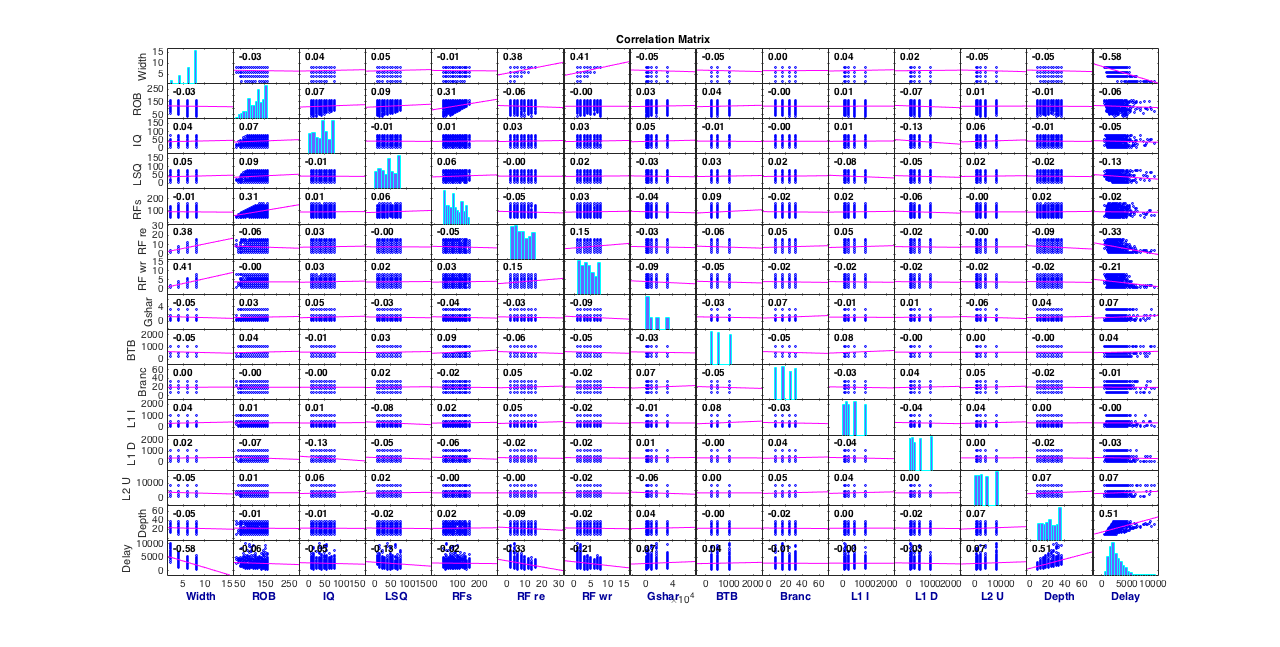
\includegraphics[width=0.8\linewidth]{covmat}
	\caption{Correlation Matrix}
	\label{fig:covmat}
\end{figure}

\section{Tools}
%Which tools and libraries have you used (e.g. Matlab, Python with scikit-learn, Java with Weka,
%Spss, language x with library y, $\ldots$). If you have source-code (Matlab scripts, Python scripts, Java source folder, \dots),
%make sure to submit it on the project website together with this report. If you only used
%command-line or GUI-tools describe what you did.

We did most of the processing using Matlab we also use R with the package \textit{randomForest 4.6-12}.

\section{Algorithm}
%Describe the algorithm you used for regression (e.g. ordinary least squares, ridge regression, $\ldots$)

\subsection*{Linear Regression}
We started by implementing a first and simple version of the linear regression to have a starting point.
Using the correlation matrix in Figure \ref{fig:covmat}, we picked some of the features to establish our model.

\subsection*{K-Fold test}

\begin{wrapfigure}{r}{0.4\linewidth}
	\centering
	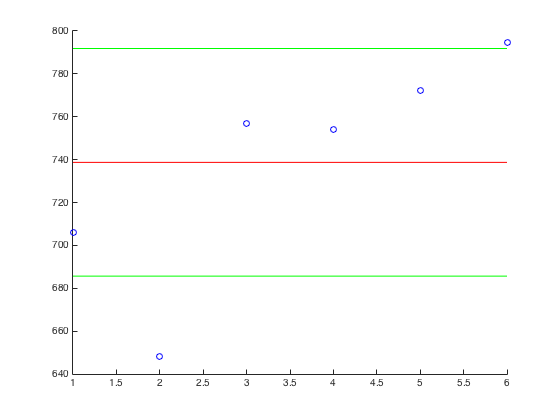
\includegraphics[width=\linewidth]{kfold}
	\caption{K-Fold test}
	\label{fig:kfold}
\end{wrapfigure}
	
In order to try different algorithm and to be sure they improved.
We implemented a \textit{K-Fold test} which compute the \textit{RMSE factor} against each $k$-part of the training set and then plotted it to have the average \textit{RMSE} and also the variance. 

\subsection*{LASSO}
We used the Matlab \textit{lassoglm} function in order to compute the regression based on LASSO.
To do so, we used also 10 cross validations and we limited the parameter $\lambda \in [3,5]$.

\subsection*{Random Forest}
We decided to implement the Random Forest algorithm in \textit{Matlab} and also in \textit{R}.
This was mainly done by 

\section{Features}
%Did you construct any new features? What feature transforms did you use?
We always started by using the linear model, and then added some of the quadratic terms for each of the algorithms.

\section{Parameters}
How did you find the parameters of your model? (What parameters have you searched over, cross validation procedure, $\ldots$)

\section{Lessons Learned} What other algorithms, tools or methods did you try out that didn't work well?
Why do you think they performed worse than what you used for your final submission?

\end{document}
